\section{External Interface Requirements}
\subsection{User Interfaces}
In this section is presented the UI of the web platform here are presented two type of user interfaces the one for the educator and the one for the student. The first one has the possibility to create tournaments and battles.
The second one has the possibility to compete inside a tournament and to receive some badges that shows the abilities that the student himself has consolidated by using the platform.Both the two types of users  need to insert their credentials to have access to the platform.Moreover a mechanism of forgot password it's needed just in case they lose their credentials. 
\subsection{Hardware Interfaces}
Our platform is a web app, as a consequence, it does not require any specific hardware interface except for computer and any other device with web browser.
\subsection{Software Interfaces}
In order to work the system needs some software  interfaces. Here they are listed in detail:
    \begin{itemize}
        \item Github API:In order to interact with github, for user login and registration as well as to create and manage repositories;
        \item Calendar API:it's useful to suggest to the user what battle it's going to happen;
        %\item Email notification:This API is useful because the user will receive a notification via email when a battle starts;
        \item Static analysis tool API: To evaluate the submitted code, we will send a request to the static tool with the code and then we expect an answer with the assigned score.
    \end{itemize}
\subsection{Communication Interfaces}
The user uses the internet connection to have access to the platform,to communicate with other user inside the platform and for pushing and pulling the code on github.The platform must be HTTPS compliant in order to work on the web properly and to be safe. 

\section{Functional Requirements}
%Definition of use case diagrams, use cases and associated sequence/activity diagrams, and mapping on requirements


\textbf{Sign up and log in}
\begin{enumerate}[label={[R\arabic*]}]
    
    \item The System allows users\footnote{users is used to refer to students and educators} to register by providing their personal information (Full Name, etc.), a valid email address and a password.
    \item The System allows registered user to log in
    \\  \\  \textbf{Tournament and battles management}
    \item The System allows Educators to create/modify a battle upload the code kata (description and software project, including test cases and build automation scripts)
    \item The System allows to create/modify/terminate a tournament by selecting the existing battles, setting the minimum and maximum number of students per group, the registration and final submission deadline.
    \item The System allows an educator to give or deny permission to his colleagues to modify a tournament.
    \item The System must notify subscribed user about upcoming battles and deadlines.
    \\  \\  \textbf{Student's teams}
    \item The System allows students to create a team
    \item The System allows students to invite other students into one of their teams
    \item The System allows students to join a new team which they were invited
    \\  \\  \textbf{Scoring and ranking}
    \item The system allows educators to define the scoring criteria for a specific battle which they have permissions to
    \item The system maintains and computes the scores of each battle
    \\ \\  \textbf{Badges}
    \item Educators can create a badge and a set of rules associated with that badge
    \item The system assigns the badges that are created by educators as a reward for the rules they fulfill
    \item The system shows the badges that are assigned to students
    \\  \\  \textbf{Tournament and battles participation}
    \item The System creates a repository on GitHub containing the code kata right after the registration deadline
    \item The system sends the link to all the enrolled students after creating the repository with the code kata
    \item The System receives notifications from GitHub regarding the students registered repositories commits
    \item The System pulls the repository after receiving a notification for that repository before the deadline of that battle
    \item The System runs the appropriate test on the new code after every pull of the repository
    \item The System calculate and update the team's score for that battle after rerunning the tests
    \\  \\  \textbf{Tournament and battles consolidation}
    \item The system updates the personal tournament score for each student enrolled in the tournament right after the battle ends
    \item The system allows educators to manually evaluate the code after the deadline
    \item The system  allows educators to finish the consolidation stage after completely performing the manual evaluation
    \item The system computes the final ranking of the tournament immediately after consolidation finishes
    \item The system  sends a notification about the tournament's termination to students 
\end{enumerate}

\subsection{Use cases Diagram}

\begin{wrapfigure}
    \centering
    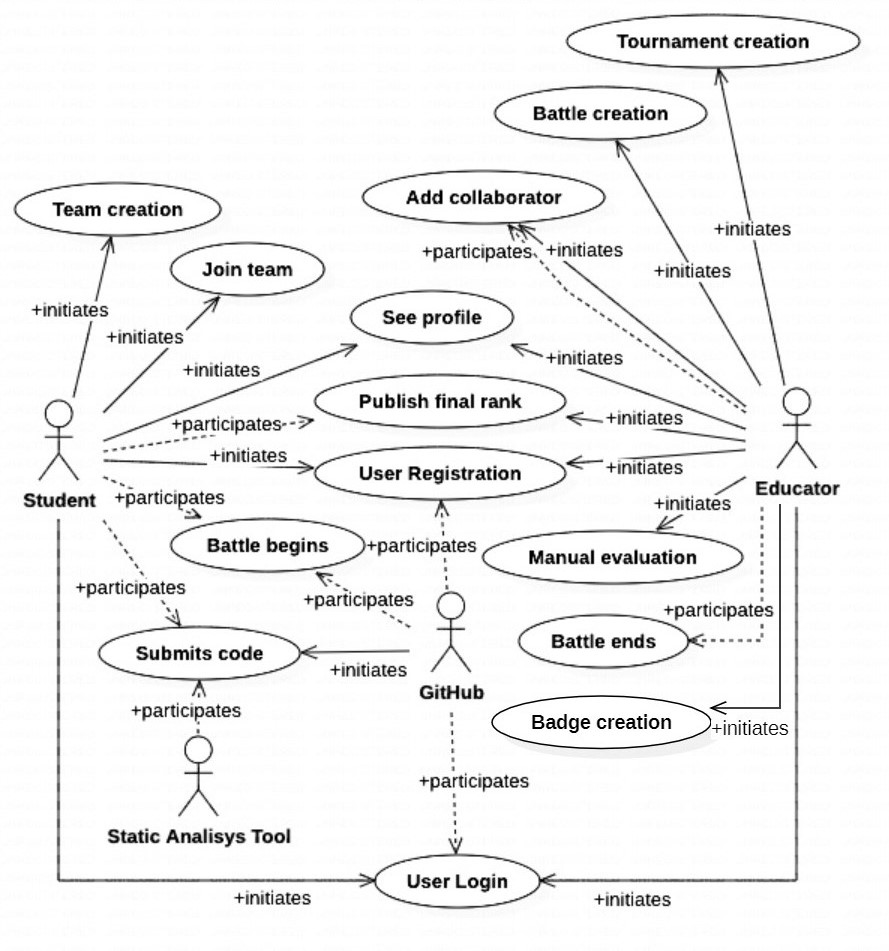
\includegraphics[width=15cm]{Images/ucd.jpg}
    \caption{Use cases diagram}
    \label{fig:enter-label}
\end{wrapfigure}

\subsection{Use cases}

\begin{enumerate}[label=\textbf{[UC\arabic*]}]
    \item \textbf{-User Registration}
    \\ \begin{tabular}{|l|p{11cm}|}
        \hline
        Name & User Registration \\
        \hline
        Actors & \begin{itemize}
                    \item user
                    \item GitHub
                \end{itemize} \\
        \hline
        Entry Condition & The user has opened the CKB platform\\
        \hline
        Event flow & \begin{enumerate} 
            \item The user press the button Sign-in
            \item The system redirect the user on GitHub to link their account to the platform
            \item The system shows a form to compile
            \item The user compile the form by adding a username
            \item The user press the button 'Register' to complete the registration
            \item The platform shows the login view
        \end{enumerate}\\
        \hline
        Exit condition & The user has successfully registered to the platform \\
        \hline
        Exception & \begin{enumerate} [label={}, leftmargin=0.25cm ]
            \item (d) There already exist a user with those credentials.
        \end{enumerate}  \\
        \hline            
    \end{tabular}
\newpage
    
 \item \textbf{-User Login}  
    \\ \begin{tabular}{|l|p{11cm}|}
        \hline
        Name & User Login\\
        \hline
        Actors & \begin{itemize}
                    \item user
                    \item GitHub
                \end{itemize} \\
        \hline
        Entry Condition & The user has opened the CKB platform\\
        \hline
        Event flow & \begin{enumerate}
            \item The user press the button Log-in
            \item The System redirect the user to GitHub platform to let him login to it, and checks the credentials
            \item The user is redirected to the platform with an access token
            \item The system shows the profile information
            \item The user presses the button 'Login'
            \item The platform shows the dashboard
        \end{enumerate}\\

        \hline
        Exit condition & The user has successfully accessed the service \\

        \hline
        Exception & \begin{enumerate} [label={}, leftmargin=0.25cm ]
            \item (c) The token is not valid. The platform will return to the entry condition
        \end{enumerate} \\ 
        \hline                
    \end{tabular}
    \pagebreak
   

    \item  \textbf{-Tournament creation}
    \\\begin{tabular}{|l|p{11cm}|}
        \hline
        Name & Tournament creation \\
        \hline
        Actors & \begin{itemize}
                    \item educator
                \end{itemize} \\
        \hline
        Entry Condition & The Educator is logged to the CKB platform\\
        \hline
        Event flow & \begin{enumerate}
            \item The educator goes to the tournament section
            \item The educator press the button to create a new tournament
            \item The system shows the educator the form to compile
            \item The educator fills the form with the information about the tournament:
            name, main context, enrolment deadline
            \item The educator press the button to submit the form
        \end{enumerate}\\
        \hline
        Exit condition & The educator has successfully created the tournament and returns to the tournament section  \\
        \hline
        Exception & \begin{enumerate} [label={}, leftmargin=0.25cm ]
            \item (d) The educator did not fill all the field of the form or they are not valid. The system will warn the user.
        \end{enumerate} \\
        \hline            
    \end{tabular}

    \newpage
    \item \textbf{-Battle creation}
        \\ \begin{tabular}{|l|p{11cm}|}
        \hline
        Name & Battle Creation \\
        \hline
        Actors & \begin{itemize}
                    \item educator
                \end{itemize} \\
        \hline
        Entry Condition & The Educator is logged to the CKB platform and he already created a tournament\\
        \hline
        Event flow & \begin{enumerate}
            \item The educator goes to the tournament where he want to add the battle
            \item The educator press the button to create a new battle
            \item The system shows the educator the form to compile
            \item The educator fills the form with the information about the battle with the following information: battle name, code template, registration deadline, final submission deadline, sets minimum and maximum number of students per group that can participate in that battle and the scoring criteria for that battle
            \item The educator press the button to submit the form
        \end{enumerate}\\
        \hline
        Exit condition & The educator has successfully created the new battle and returns to the tournament main page \\
        \hline
        Exception & \begin{enumerate} [label={}, leftmargin=0.25cm ]
            \item (d) The educator did not fill all the field of the form or they are not valid. The system will warn the user. 
        \end{enumerate}\\
        \hline            
    \end{tabular}

\item \textbf{-Add collaborator}
    \\ \begin{tabular}{|l|p{11cm}|}
        \hline
        Name & Add collaborator\\
        \hline
        Actors & \begin{itemize}
                    \item educator
                \end{itemize} \\
        \hline
        Entry Condition & The educator is logged to the CKB platform and he is in the tournament section\\
        \hline
        Event flow & \begin{enumerate}
            \item The educator select the tournament
            \item The educator press the button to share the control of a tournament
            \item The system shows the educator a bar where to search other educators
            \item The educator can choose the other educators
            
        \end{enumerate}\\
        \hline
        Exit condition & The educator has successfully shared the access to the tournament control  \\
        \hline
        Exception & \begin{enumerate} [label={}, leftmargin=0.25cm ]
            \item (d) The educator did not make the correct choice
        \end{enumerate} \\
        \hline            
    \end{tabular}

\newpage
\item  \textbf{-Team creation}
    \\ \begin{tabular}{|l|p{11cm}|}
        \hline
        Name & Team creation \\
        \hline
        Actors & \begin{itemize}
                    \item student
                \end{itemize} \\
        \hline
        Entry Condition & The student is logged to the CKB platform and is enrolled into a tournament\\
        \hline
        Event flow & \begin{enumerate}
            \item The student goes to tournament section and selects the tournament
            \item The student select the battle for which create the team
            \item The student press the button create a team
            \item The system shows the student the form to compile
            \item The student fills the form with the information about the team: team name
            \item The system generate the link of the team 
            \item The student shares the link of the team with his friends
        \end{enumerate}\\
        \hline
        Exit condition &  The link team is successfully generated \\
        \hline
        Exception & \begin{enumerate} [label={}, leftmargin=0.25cm ]
            \item (c) The student has already created a team for that battle
        \end{enumerate} \\
        \hline            
    \end{tabular}

\item  \textbf{-Join team}
    \\ \begin{tabular}{|l|p{11cm}|}
        \hline
        Name & Join team  \\
        \hline
        Actors & \begin{itemize}
                    \item student
                \end{itemize} \\
        \hline
        Entry Condition & The student has the link to join a team\\
        \hline
        Event flow & \begin{enumerate}
            \item The student opens the link received
            \item The system checks the student's credentials
            \item The student press the button 'join the team'
            \item The system checks if the team is not full and that the student is not already enrolled in the battle
            \item The system redirect the student into the team dashboard
        \end{enumerate}\\
        \hline
        Exit condition &   The student has correctly joined the team \\
        \hline
        Exception & \begin{enumerate} [label={}, leftmargin=0.25cm ]
            \item (b) The student is not logged in, he will be redirect to the log in page
            \item (d) The system returns an error message
        \end{enumerate}\\ 
        \hline            
    \end{tabular}
\newpage
    \item  \textbf{-Battle begins}
    \\ \begin{tabular}{|l|p{11cm}|}
        \hline
        Name & Battle begins \\
        \hline
        Actors & \begin{itemize} 
                    \item student
                    \item GitHub
                \end{itemize} \\
        \hline
        Entry Condition & The enrollment deadline of the battle ended\\
        \hline
        Event flow & \begin{enumerate}
            \item The system creates a GitHub repository by using the appropriate API call for every enrolled team enrolled
            \item The system sends a notification to the students enrolled to the battle with the link to the specifically created repository for them to fork
        \end{enumerate}\\
        \hline
        Exit condition &   The code is available to all the students participating\\
        \hline
        Exception & \begin{enumerate} [label={}, leftmargin=0.25cm ]
            \item (b) The notification is not correctly sent, the system will retry to send it later.
        \end{enumerate}\\ 
        \hline            
    \end{tabular}

 \item  \textbf{-Submits code}
    \\ \begin{tabular}{|l|p{11cm}|}
        \hline
        Name & Student pushes the code \\
        \hline
        Actors & \begin{itemize}
                    \item student
                    \item GitHub
                    \item Static analysis tool
                \end{itemize} \\
        \hline
        Entry Condition & The student has forked to the git hub repository provided by the platform and set up the automated workflow. The student has committed the code into their GitHub repository\\
        \hline
        Event flow & \begin{enumerate}
            \item The system is triggered by GitHub about a new commit
            \item The system dynamically evaluates the code by running the test on it.
            \item The system send the code to the static analysis tool 
            \item The system receives the evaluation by the tool
            \item The system updates the score of the team.
        \end{enumerate}\\
        \hline
        Exit condition &   The scoring rank is correctly updated\\
        \hline
        Exception & \begin{enumerate} [label={}, leftmargin=0.25cm ]
             \item (a) The repository is not a fork of a code kata team, the system will ignore it and log it.
            \item (a) The system is triggered after the deadline of the battle, it will not evaluate the code and send a notification to the team warning them 
           
        \end{enumerate}\\ 
        \hline            
    \end{tabular}
\newpage
    \item  \textbf{-The battle ends}
    \\ \begin{tabular}{|l|p{11cm}|}
        \hline
        Name & The battle ends \\
        \hline
        Actors & \begin{itemize}
                    \item educator
                \end{itemize} \\
        \hline
        Entry Condition & the battle deadline has expired \\
        \hline
        Event flow & \begin{enumerate}
            \item The system creates the rank of the battle
            \item The system sends a notification the the educators enrolled into the battle about the end of it
        \end{enumerate}\\
        \hline
        Exit condition & The ranking is available on the platform \\
        \hline
        Exception & \begin{enumerate} [label={}, leftmargin=0.25cm ]
            \item (b) The notification is not correctly sent, the system will notify it and retry to send it
        \end{enumerate}\\ 
        \hline            
    \end{tabular}

        \item  \textbf{-Code evaluation}
    \\ \begin{tabular}{|l|p{11cm}|}
        \hline
        Name & The code is evaluated \\
        \hline
        Actors & \begin{itemize}
                    \item educator
                \end{itemize} \\
        \hline
        Entry Condition & The tournament ended, the consolidation phase started and the educator is logged to the CKB platform\\
        \hline
        Event flow & \begin{enumerate}
            \item The educator goes to the tournament section
            \item The educator select the tournament which needs a manual evaluation
            \item The educator reads the sources produced by the teams
            \item The educator assign a score to each student enrolled to the battle
        \end{enumerate}\\
        \hline
        Exit condition &  The system stores the score provided by the educator\\
        
        \hline            
    \end{tabular}
\newpage
        \item  \textbf{-Publish final rank}
    \\ \begin{tabular}{|l|p{11cm}|}
        \hline
        Name & Final rank made available \\
        \hline
        Actors & \begin{itemize}
                    \item student
                    \item educator
                \end{itemize} \\
        \hline
        Entry Condition & The tournament is in consolidation phase, the educator is logged to the CKB platform \\
        \hline
        Event flow & \begin{enumerate}
            \item The educator goes to the tournament section
            \item The educator selects the tournament to close
            \item The educator press the button 'close the tournament'
            \item The system computes the final rank for each student enrolled into the tournament
            \item The system notifies the student about the availability of the rank
            \item The system checks among the participating students who satisfied the badges requirement
            \item The system assign the badge to the students
        \end{enumerate}\\
        \hline
        Exit condition &  The final rank is published, and badges has been assigned \\
        \hline
        Exception & \begin{enumerate}  [label={}, leftmargin=0.25cm ]
            \item (c) If any student does not have a manual evaluation and it was required then an error message will be shown.
            \item (e) The notification is not correctly sent, the system will notify it and retry to send it
        \end{enumerate}\\ 
        \hline            
    \end{tabular}


        \item  \textbf{-See profile}
    \\ \begin{tabular}{|l|p{11cm}|}
        \hline
        Name & see profile \\
        \hline
        Actors & \begin{itemize}
                    \item user
                \end{itemize} \\
        \hline
        Entry Condition &  The user is logged to the CKB platform\\
        \hline
        Event flow & \begin{enumerate}
            \item The user search the name of the student
            \item The system shows the list
            \item The user selects the Student
        \end{enumerate}\\
        \hline
        Exit condition & The platform shows the rank of the selected student  
        \\
        \hline
        Exception & \begin{enumerate} [label={}, leftmargin=0.25cm ]
            \item (a) The person searched  does not match with any user in the system. It shows a no student found message
        \end{enumerate}\\ 
        \hline            
    \end{tabular}

\newpage

 \item \textbf{-Badge creation}
    \\ \begin{tabular}{|l|p{11cm}|}
        \hline
        Name & Badge Creation \\
        \hline
        Actors & \begin{itemize}
                    \item educator
                \end{itemize} \\
        \hline
        Entry Condition & The educator is logged on to the CKB platform and he already created a tournament\\
        \hline
        Event flow & \begin{enumerate}
            \item The educator goes to tournament section
            \item The educator goes to the tournament where he want to add the badge
            \item The educator press the button to create a new badge
            \item The system shows the educator the form to compile
            \item The educator fills the form with the information about the badge with the following information: badge name and the rule which has to comply with the syntax specified $^2$
            \item The educator press the button to submit the form
        \end{enumerate}\\
        \hline
        Exit condition & The educator has successfully created the new badge and returns to the tournament main page \\
        \hline
        Exception & \begin{enumerate} [label={}, leftmargin=0.25cm ]
            \item (e) The educator did not fill all the field of the form or they are not valid  (e.g. the rule is invalid). The system will warn the user. 
        \end{enumerate}\\
        \hline            
    \end{tabular}
    \footnote{More details on the rules syntax will be provided in the DD}
\end{enumerate}
\newpage

\subsection{Sequence diagrams}

\begin{enumerate}[label=\textbf{[UC\arabic*]}]

    \begin{figure}[!h]
    \item \textbf{User Registration}
    \centering
    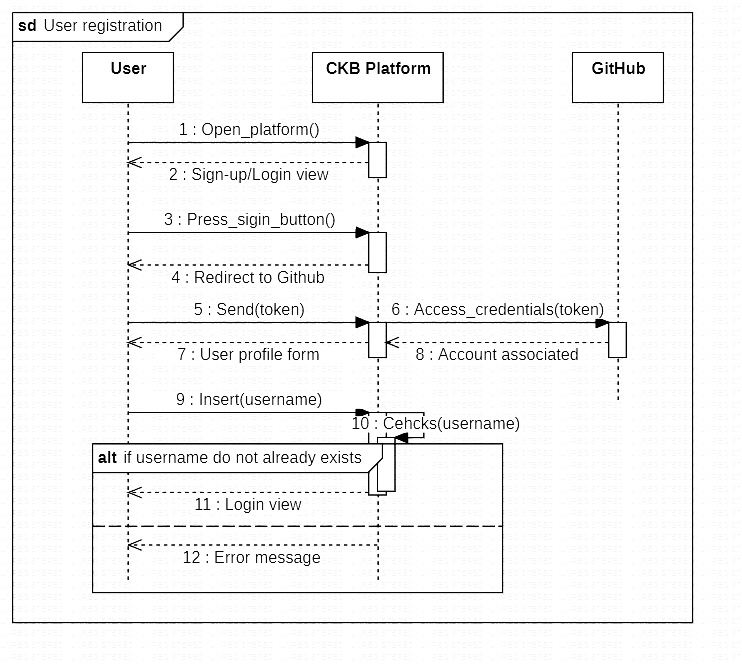
\includegraphics[width=\textwidth]{Images/User registration.jpg}
    \caption{User Registration}
    \label{fig:enter-label}
    \end{figure}

    \begin{figure}
    \item \textbf{User Login}
    \centering
    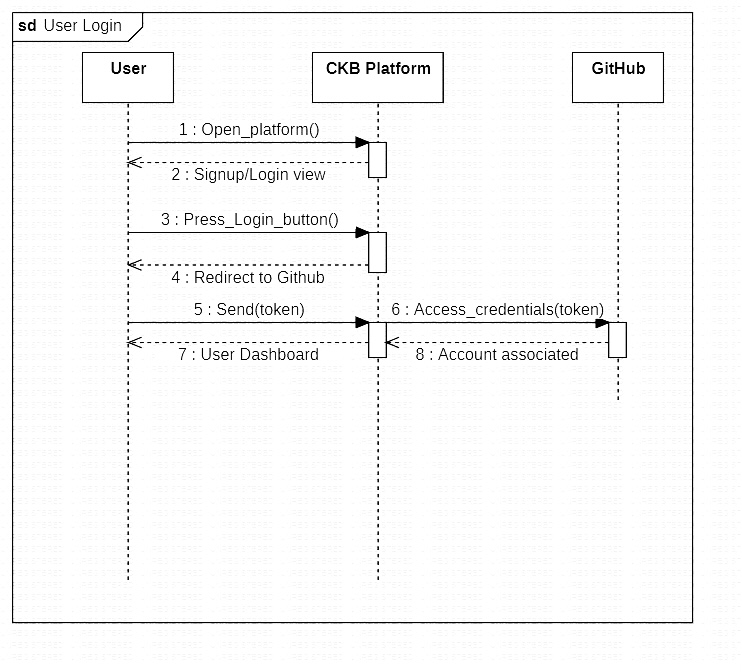
\includegraphics[width= \textwidth]{Images/User login.jpeg}
    \caption{User Login}
    \label{fig:enter-label}
    \end{figure}



    \begin{figure}
    \item \textbf{Tournament Creation}
        \centering
        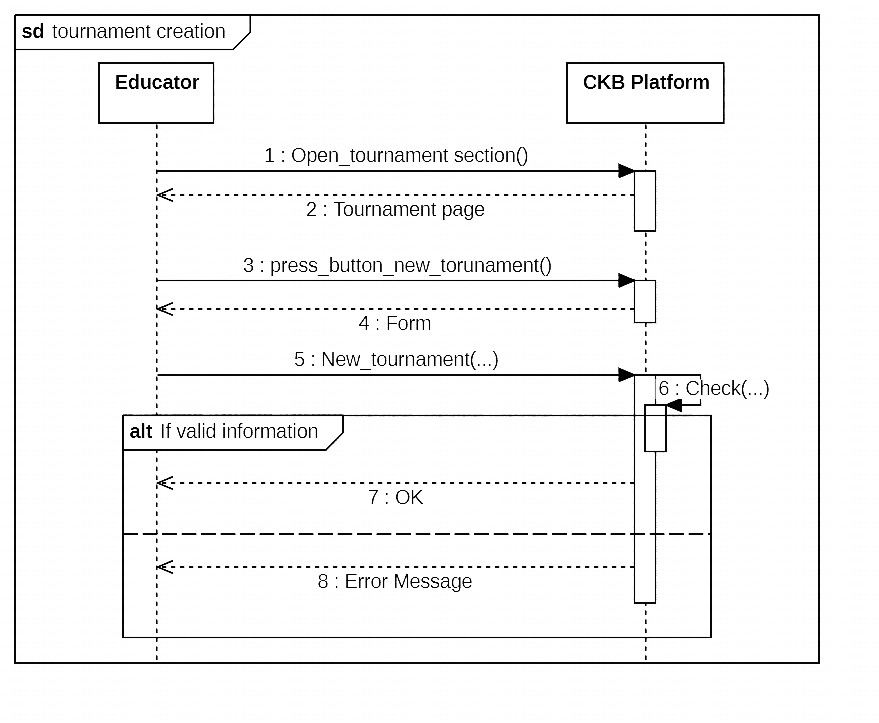
\includegraphics[width= \textwidth]{Images/Tournament creation.jpg}
        \caption{Tournament Creation}
        \label{fig:enter-label}
    \end{figure}
    
    
    \begin{figure}
    \item \textbf{Battle Creation}
        \centering
        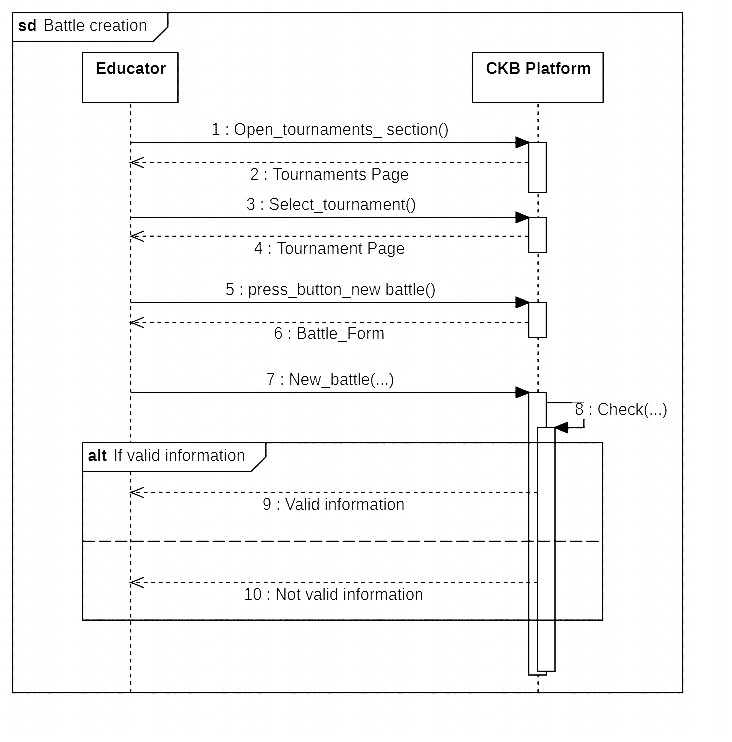
\includegraphics[width= \textwidth]{Images/Battle creation.jpg}
        \caption{Battle Creation}
        \label{fig:enter-label}
    \end{figure}
    
    \begin{figure}
    \item \textbf{Add collaborator}
        \centering
        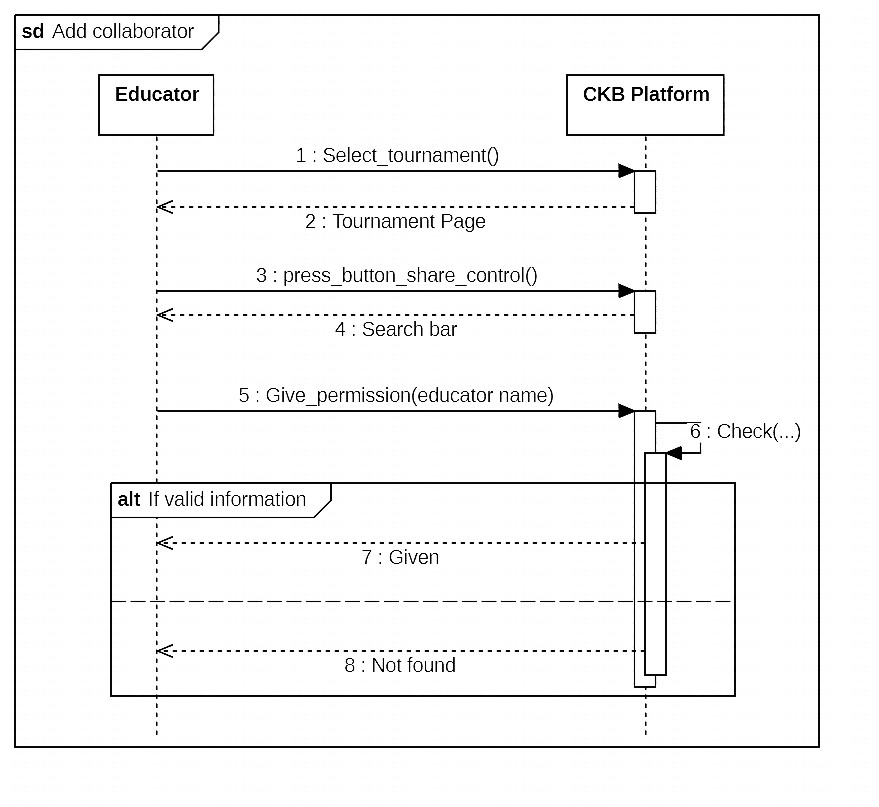
\includegraphics[width= \textwidth]{Images/Add collaborator.jpg}
        \caption{Add collaborator}
        \label{fig:enter-label}
    \end{figure}
    
    
    \begin{figure}
    \item \textbf{Team Creation}
        \centering
        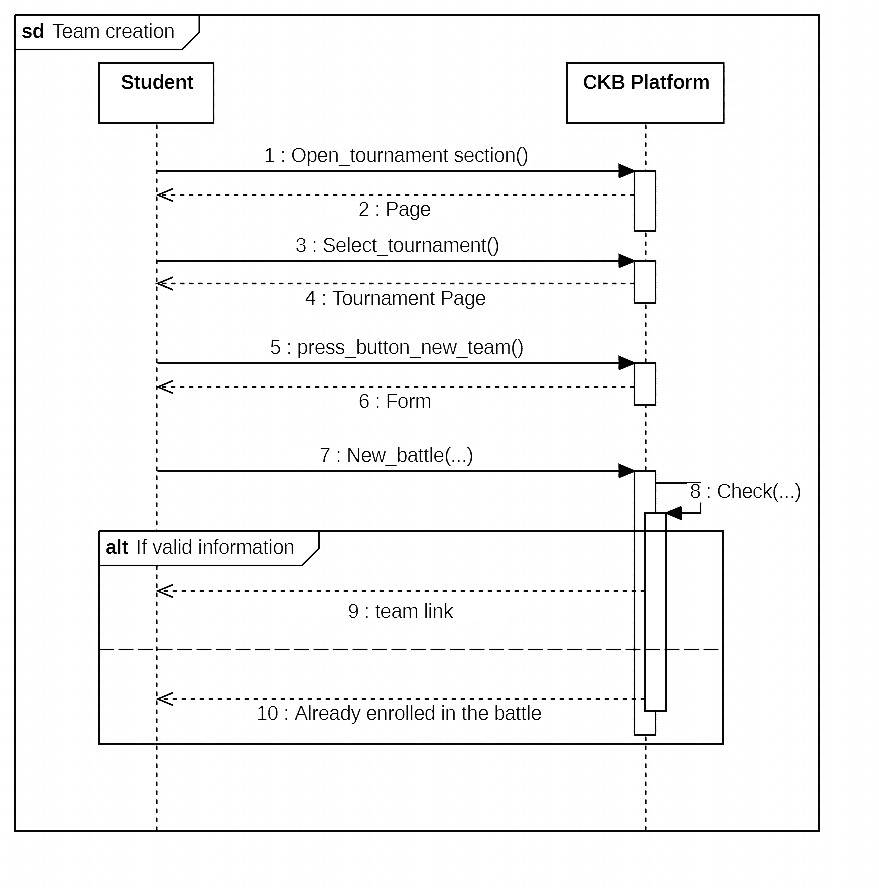
\includegraphics[width= \textwidth]{Images/Team creation.jpg}
        \caption{Team Creation}
        \label{fig:enter-label}
    \end{figure}
    
    \begin{figure}
    \item \textbf{Join Team}
        \centering
        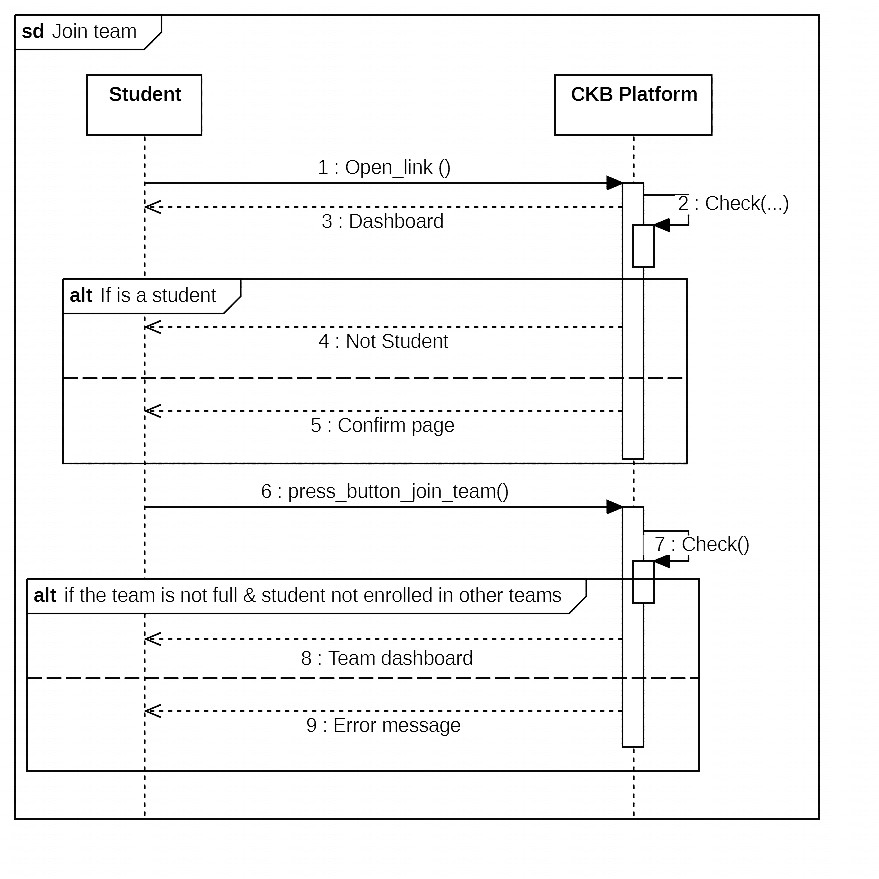
\includegraphics[width= \textwidth]{Images/Join team.jpg}
        \caption{Join Team}
        \label{fig:enter-label}
    \end{figure}
    
    \begin{figure}
    \item \textbf{Battle Begins}
        \centering
        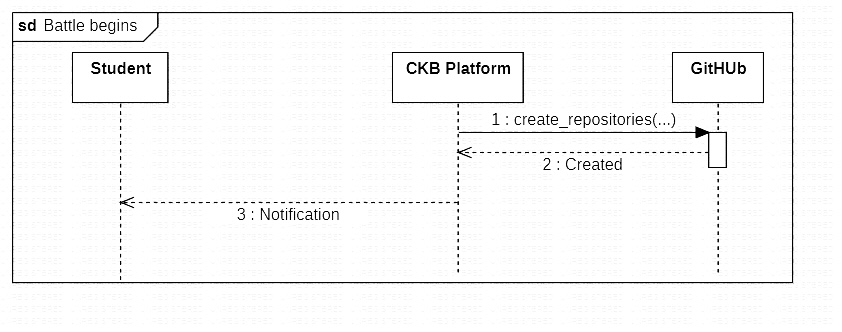
\includegraphics[width= \textwidth]{Images/Battle begins.jpg}
        \caption{Battle Begins}
        \label{fig:enter-label}
    \end{figure}
    
    \begin{figure}
    \item \textbf{Submits code}
        \centering
        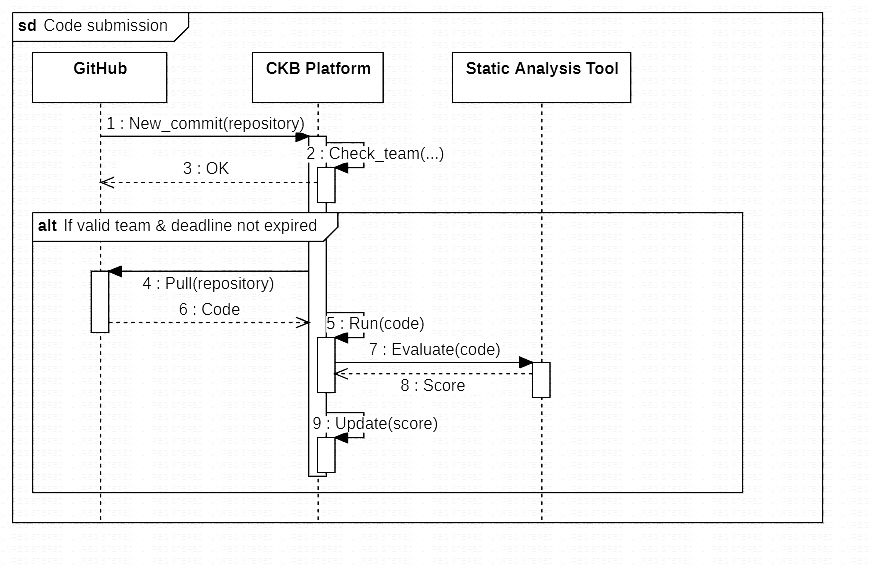
\includegraphics[width= \textwidth]{Images/Code submission.jpg}
        \caption{Submits Code}
        \label{fig:enter-label}
    \end{figure}

    \begin{figure}
    \item \textbf{The battle ends}
        \centering
        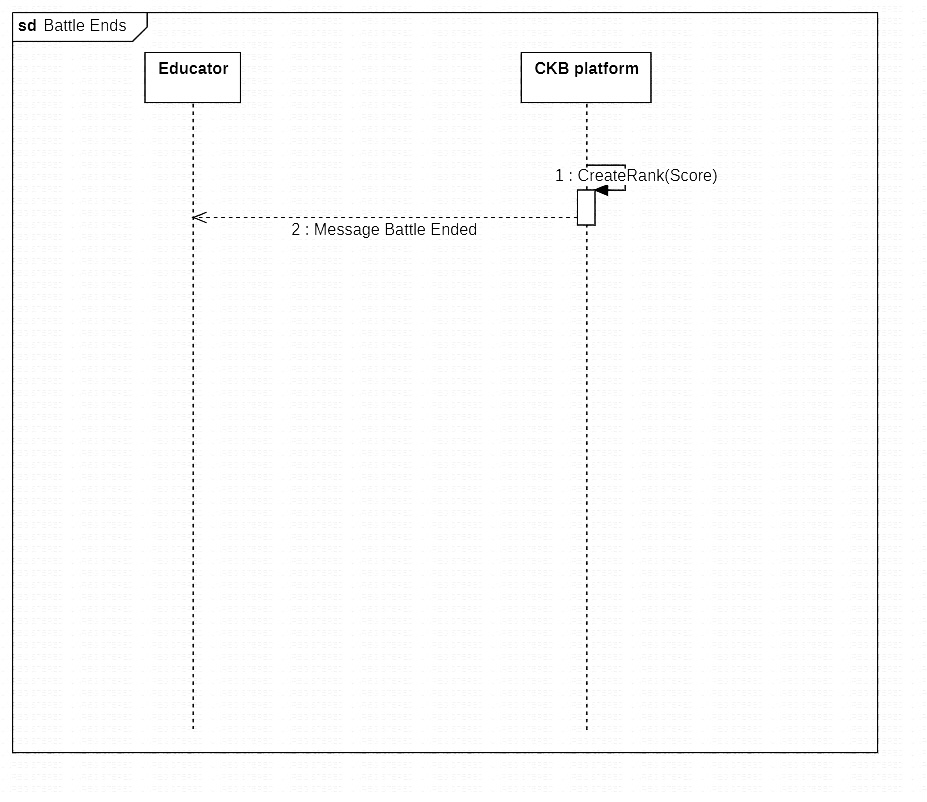
\includegraphics[width= \textwidth]{Images/Battle Ends.jpg}
        \caption{The battle ends}
        \label{fig:enter-label}
    \end{figure}
    
    \begin{figure}
    \item \textbf{Code Evaluation}
        \centering
        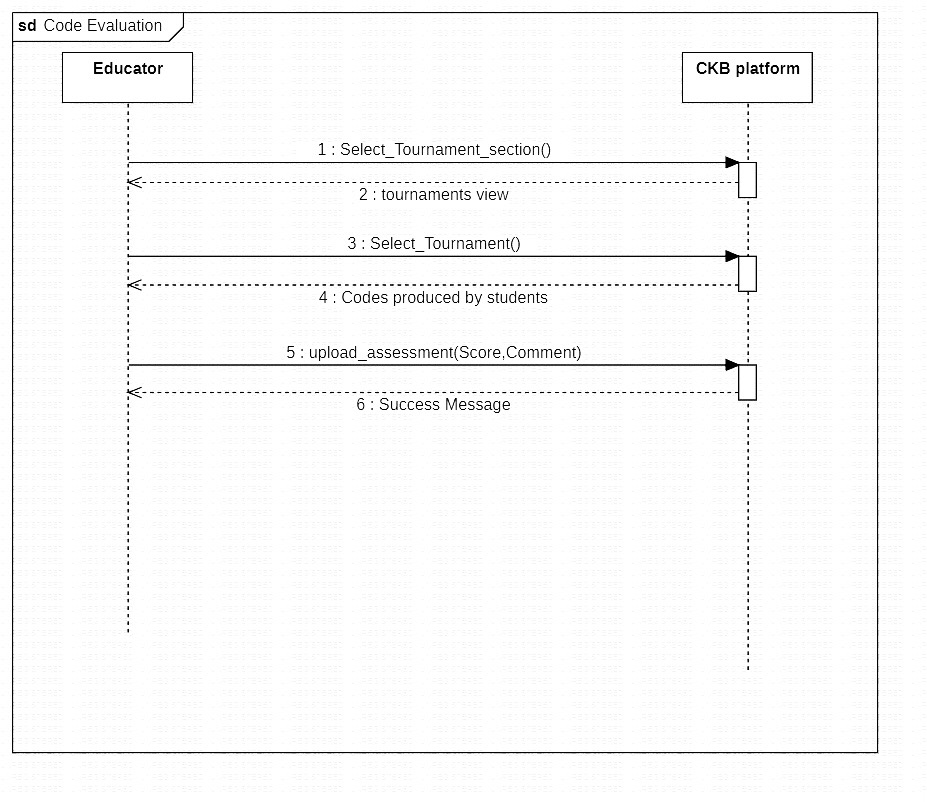
\includegraphics[width= \textwidth]{Images/f4c0a22a-3bab-4ba7-8605-08f8577774b5}
        \caption{Code Evaluation}
        \label{fig:enter-label}
    \end{figure}
    
    \begin{figure}
    \item \textbf{Publish Final Rank}
        \centering
        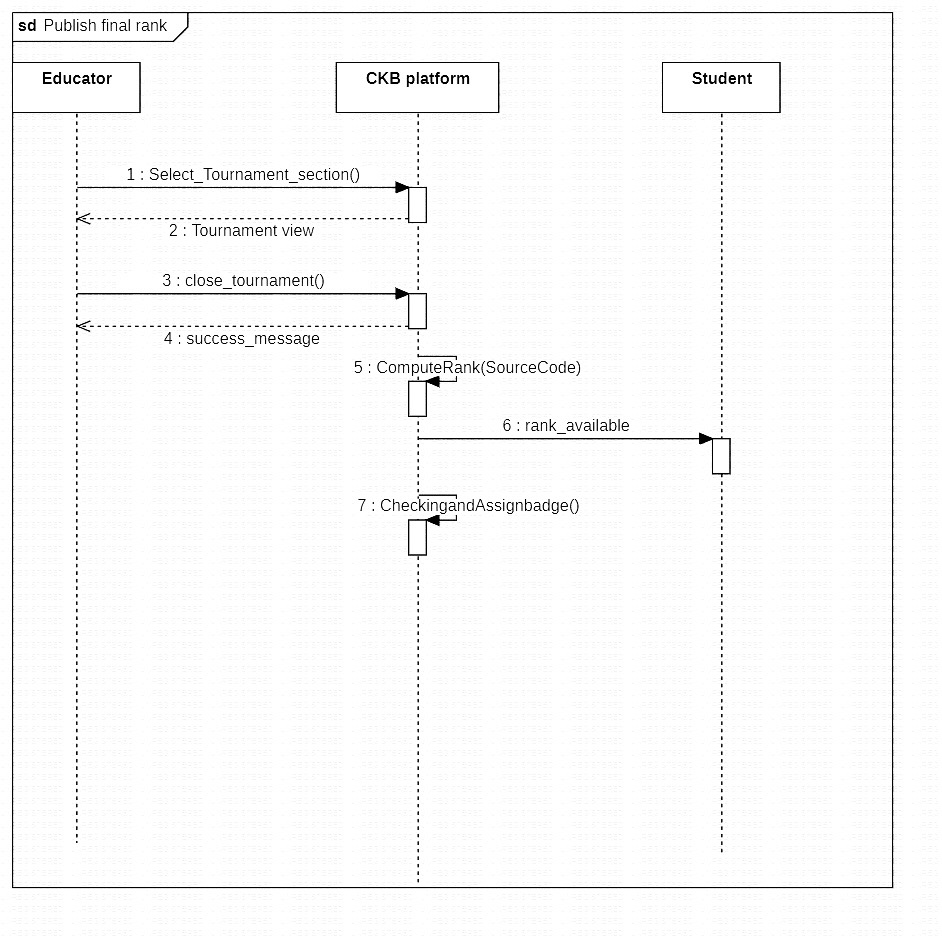
\includegraphics[width= \textwidth]{Images/e08ea53b-0385-4fb7-8284-6672fda72856}
        \caption{Publish Final Rank}
        \label{fig:enter-label}
    \end{figure}

    \begin{figure}
    \item \textbf{See Profile}
        \centering
        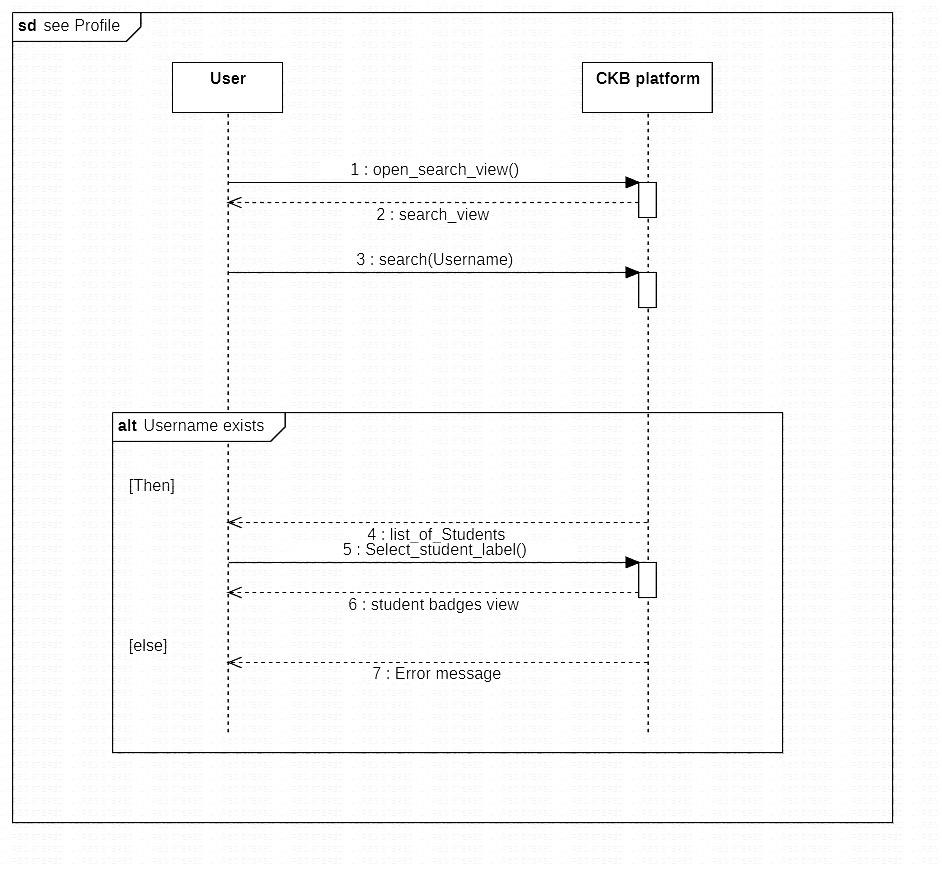
\includegraphics[width= \textwidth]{Images/WhatsApp Image 2023-12-20 at 18.34.43_e728ecf8.jpg}
        \caption{See Profile}
        \label{fig:enter-label}
    \end{figure}

    \begin{figure}
    \item \textbf{Badge Creation}
        \centering
        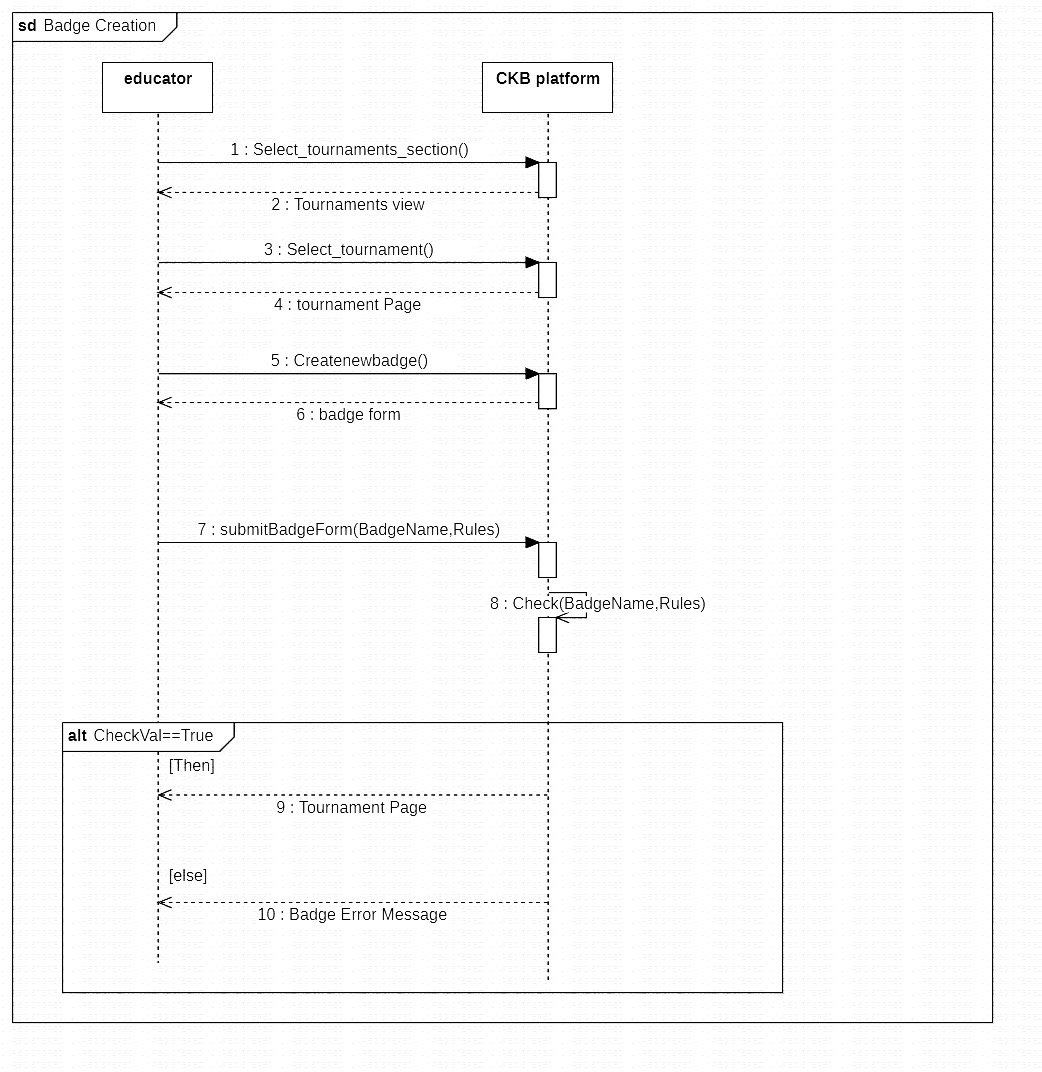
\includegraphics[width= \textwidth]{2058f325-4760-4dfa-ad83-44ce21cc7063}
        \caption{Badge Creation}
        \label{fig:enter-label}
    \end{figure}

    

    
    
\end{enumerate}








\pagebreak[4]
\newpage

\subsection{Requirement mapping}
\begin{tabular}{|p{7cm}|p{7cm}|}
\hline
\multicolumn{2}{|c|}{
\textbf{[G1] Educators create code kata battles} }
\\
\hline
\begin{itemize} 
\item [R1] The System allows users1 to register by providing their personal information (Full Name, etc.), a valid email address and a password
\item [R2] The System allows registered user to log in
\item [R3] The System allows Educators to create/modify a battle upload the code kata (description and software project, including test cases and build automation scripts)
\item [R4] The System allows to create/modify/terminate a tournament by selecting the existing battles, setting the minimum and maximum number of students per group, the registration and final submission deadline.
\item [R5] The System allows an educator to give or deny permission to his colleagues to modify a tournament.
\item [R10] The system allows educators to define the scoring criteria for a specific battle which they have permissions to
\item [R11] The system maintains and computes the scores of each battle
\item [R12] Educators can create a badge and a set of rules associated with that badge
\end{itemize}
&
\begin{itemize}
    \item [D1] User must have a reliable internet connection
    \item [D2] User personal information must be correct
    \item [D3] Educators properly insert information about a tournament
    \item [D7] The educator correctly adds information about a new badge such as new rules or badge name
\end{itemize}
\\
\hline
\end{tabular}

\pagebreak

\begin{tabular}{|p{7cm}|p{7cm}|}
\hline
\multicolumn{2}{|c|}{
\textbf{[G2] Students compete in multiple tournaments in teams} }
\\
\hline
\begin{itemize}
    \item [R1] The System allows users to register using a github acccount
    \item [R2] The System allows registered user to log in
    \item [R6] The System must notify subscribed user about upcoming battles and deadlines.
    \item [R7] The System allows students to create a team
    \item [R8] The System allows students to invite other students into one of their teams
    \item [R9] The System allows students to join a new team which they were invited
    \item [R15] The System creates a repository on GitHub containing the code kata right after the registration deadline
    \item [R16] The system sends the link to all the enrolled students after creating the repository with the code kata
    \item [R17] The System receives notifications from GitHub regarding the students registered repositories commits
    \item [R18] The System pulls the repository after receiving a notification for that repository before the deadline of that battle
    \item [R19] The System runs the appropriate test on the new code after every pull of the repository
    \item [R20] The System calculate and update the team's score for that battle after rerunning the tests
    \item [R25] The system  sends a notification about the tournament's termination to students
\end{itemize}
&
\begin{itemize}
    \item [D1] User must have a reliable internet connection
    \item [D2] User personal information must be correct
    \item [D4] The Github interaction it's reliable( the user is able to pull and push the code without losing its data)
    \item [D5] Notifications to the user must arrive as soon as the final rank is available
\end{itemize}
\\
\hline
\end{tabular}

\begin{tabular}{|p{7cm}|p{7cm}|}
\hline
\multicolumn{2}{|c|}{
\textbf{[G3] Students receive performance feedback after each battle assessment}}
\\
\hline
\begin{itemize}
    \item [R10] The system allows educators to define the scoring criteria for a specific battle which they have permissions to
    \item [R11] The system maintains and computes the scores of each battle
    \item [R12] Educators can create a badge and a set of rules associated with that badge
    \item[R13] The system assigns the badges that are created by educators as a reward for the rules they fulfill
    \item [R14] The system shows the badges that are assigned to students 
    \item [R20] The System calculate and update the team's score for that battle after rerunning the tests
    \item [R21] The system updates the personal tournament score for each student enrolled in the tournament right after the battle ends
    \item [R22] The system allows educators to manually evaluate the code after the deadline
    \item [R23] The system  allows educators to finish the consolidation stage after completely performing the manual evaluation
    \item [R24] The system computes the final ranking of the tournament immediately after consolidation finishes
\end{itemize}
&
\begin{itemize}
    \item [D4] The Github interaction it's reliable( the user is able to pull and push the code without losing its data)
    \item [D5] Notifications to the user must arrive as soon as the final rank is available
    \item [D6] The Educator properly insert an evaluation manually when it’s requested
    \item [D7] The educator correctly adds information about a new badge such as new rules or badge name
\end{itemize}
\\
\hline
\end{tabular}



\section{Performance Requirements}
The system has to guarantee good performances in order to serve a great number of users (educators and students).To achieve this goal the user experience must be as good as possible in order to fulfill this requirement the response time must be low no more than a second.If the user’s internet connection is slow the response time can increase  enormously

\section{Design Constraints}

\subsection{Standards compliance}
The CKB platform pays a great attention for what concerns users privacy cause of this the CKB project is in compliance with the  General Data Protection Regulation
(GPDR) a regulation in EU law on data protection and privacy for all
individuals within the European Union (EU) and the European Economic Area (EEA).
Moreover, the platform has to use the international format of date and time to adequate to the newer standards.
\subsection{Hardware limitations}
Here is presented a summary of the hardware features that a user should have to use the platform properly:
    \begin{enumerate}[label=\textbullet]
        \item The user must have a device with a good internet connection for providing this the device should be compatible with at least one of this standards 3G, 4G, 5G, IEEE 802.11 and  IEEE 802.3. Both for the wired and wireless communications it must be connected to a device able to guarantee an internet connection such as a modem or an access point and so on;
        \item The user must have a device with good hardware features such as a processor with high performance as an example intel i5 or i7 and a display with high resolution at least full hd and a fair amount of ram at least 8 GB.
        
    \end{enumerate}



    


\subsection{Any other constraint}
The UI should be user-friendly because the CKB platform is developed for educators and students that are learning to code. Furthermore, they must be able to use the platform in a simple and efficient way.

\section{Software System Attributes}
Here are explained some  software side attributes that the system should provide.
\subsection{Reliability}
The system has to be reliable because it will have to run continuously for a long period of time.
To ensure this feature the platform must have some sort of replication and consistency policy to avoid system crash. Moreover, as best practice, it is important to have offline backups of the system for recovering information after data loss.
\subsection{Availability}
The most important attribute that the system has to provide is the availability. The system should have an availability of 99\%.Since the platform has to achieve this goal some replication policies must be implemented and a single point of failure should be avoided. Also it has to be specially prepared for a possibly large amount of submissions when deadline is close.
\subsection{Security}
The system will store the users personal data so the security aspect must be carefully considered. Passwords stored in the central database must be encrypted.
The data store must be protected with all possible security measures to avoid internal and external attacks. The CKB platform must ensure integrity, consistency and confidentiality by using appropriate cyber-risk avoidance policies.
Additionally, because students code will be ran on the system for the dynamic analysis, a proper way to do these has to be explored making sure no malicious code can  damage the platform.
\subsection{Maintainability}The system must guarantee a good level of maintainability. The code has to be well documented. A testing routine has to be provided and it has to cover at least 75\% of the entire code excluding the UI code.
\subsection{Portability}
The system is a web application so it must be compatible with different web browser (Firefox,Google Chrome and so on) and devices (smartphones, computers, etc).



